  % begin the content of the document
\sloppy  % this to relax whitespacing in favour of straight margins


% title on top of the document
\maintitle{Keagan Thompson}{April 16, 1994}{Last update on \today}

\nobreakvspace{0.3em}  % add some page break averse vertical spacing

\noindent\href{mailto:u13023782.at.gmail.dot.com}{u13023782\mbox{}@\mbox{}gmail.com}\sbull
\textsmaller{+}27.822182880\sbull
\\
216 The Circuits\sbull
1228 Prospect Street\sbull
Hatfield\sbull
Pretoria\\

\spacedhrule{0.9em}{-0.4em}  % a horizontal line with some vertical spacing before and after
\begin{center}
\roottitle{Summary}  % a root section title
\end{center}


\vspace{-1.3em}  % some vertical spacing
\begin{multicols}{3}% open a multicolumn environment

\noindent 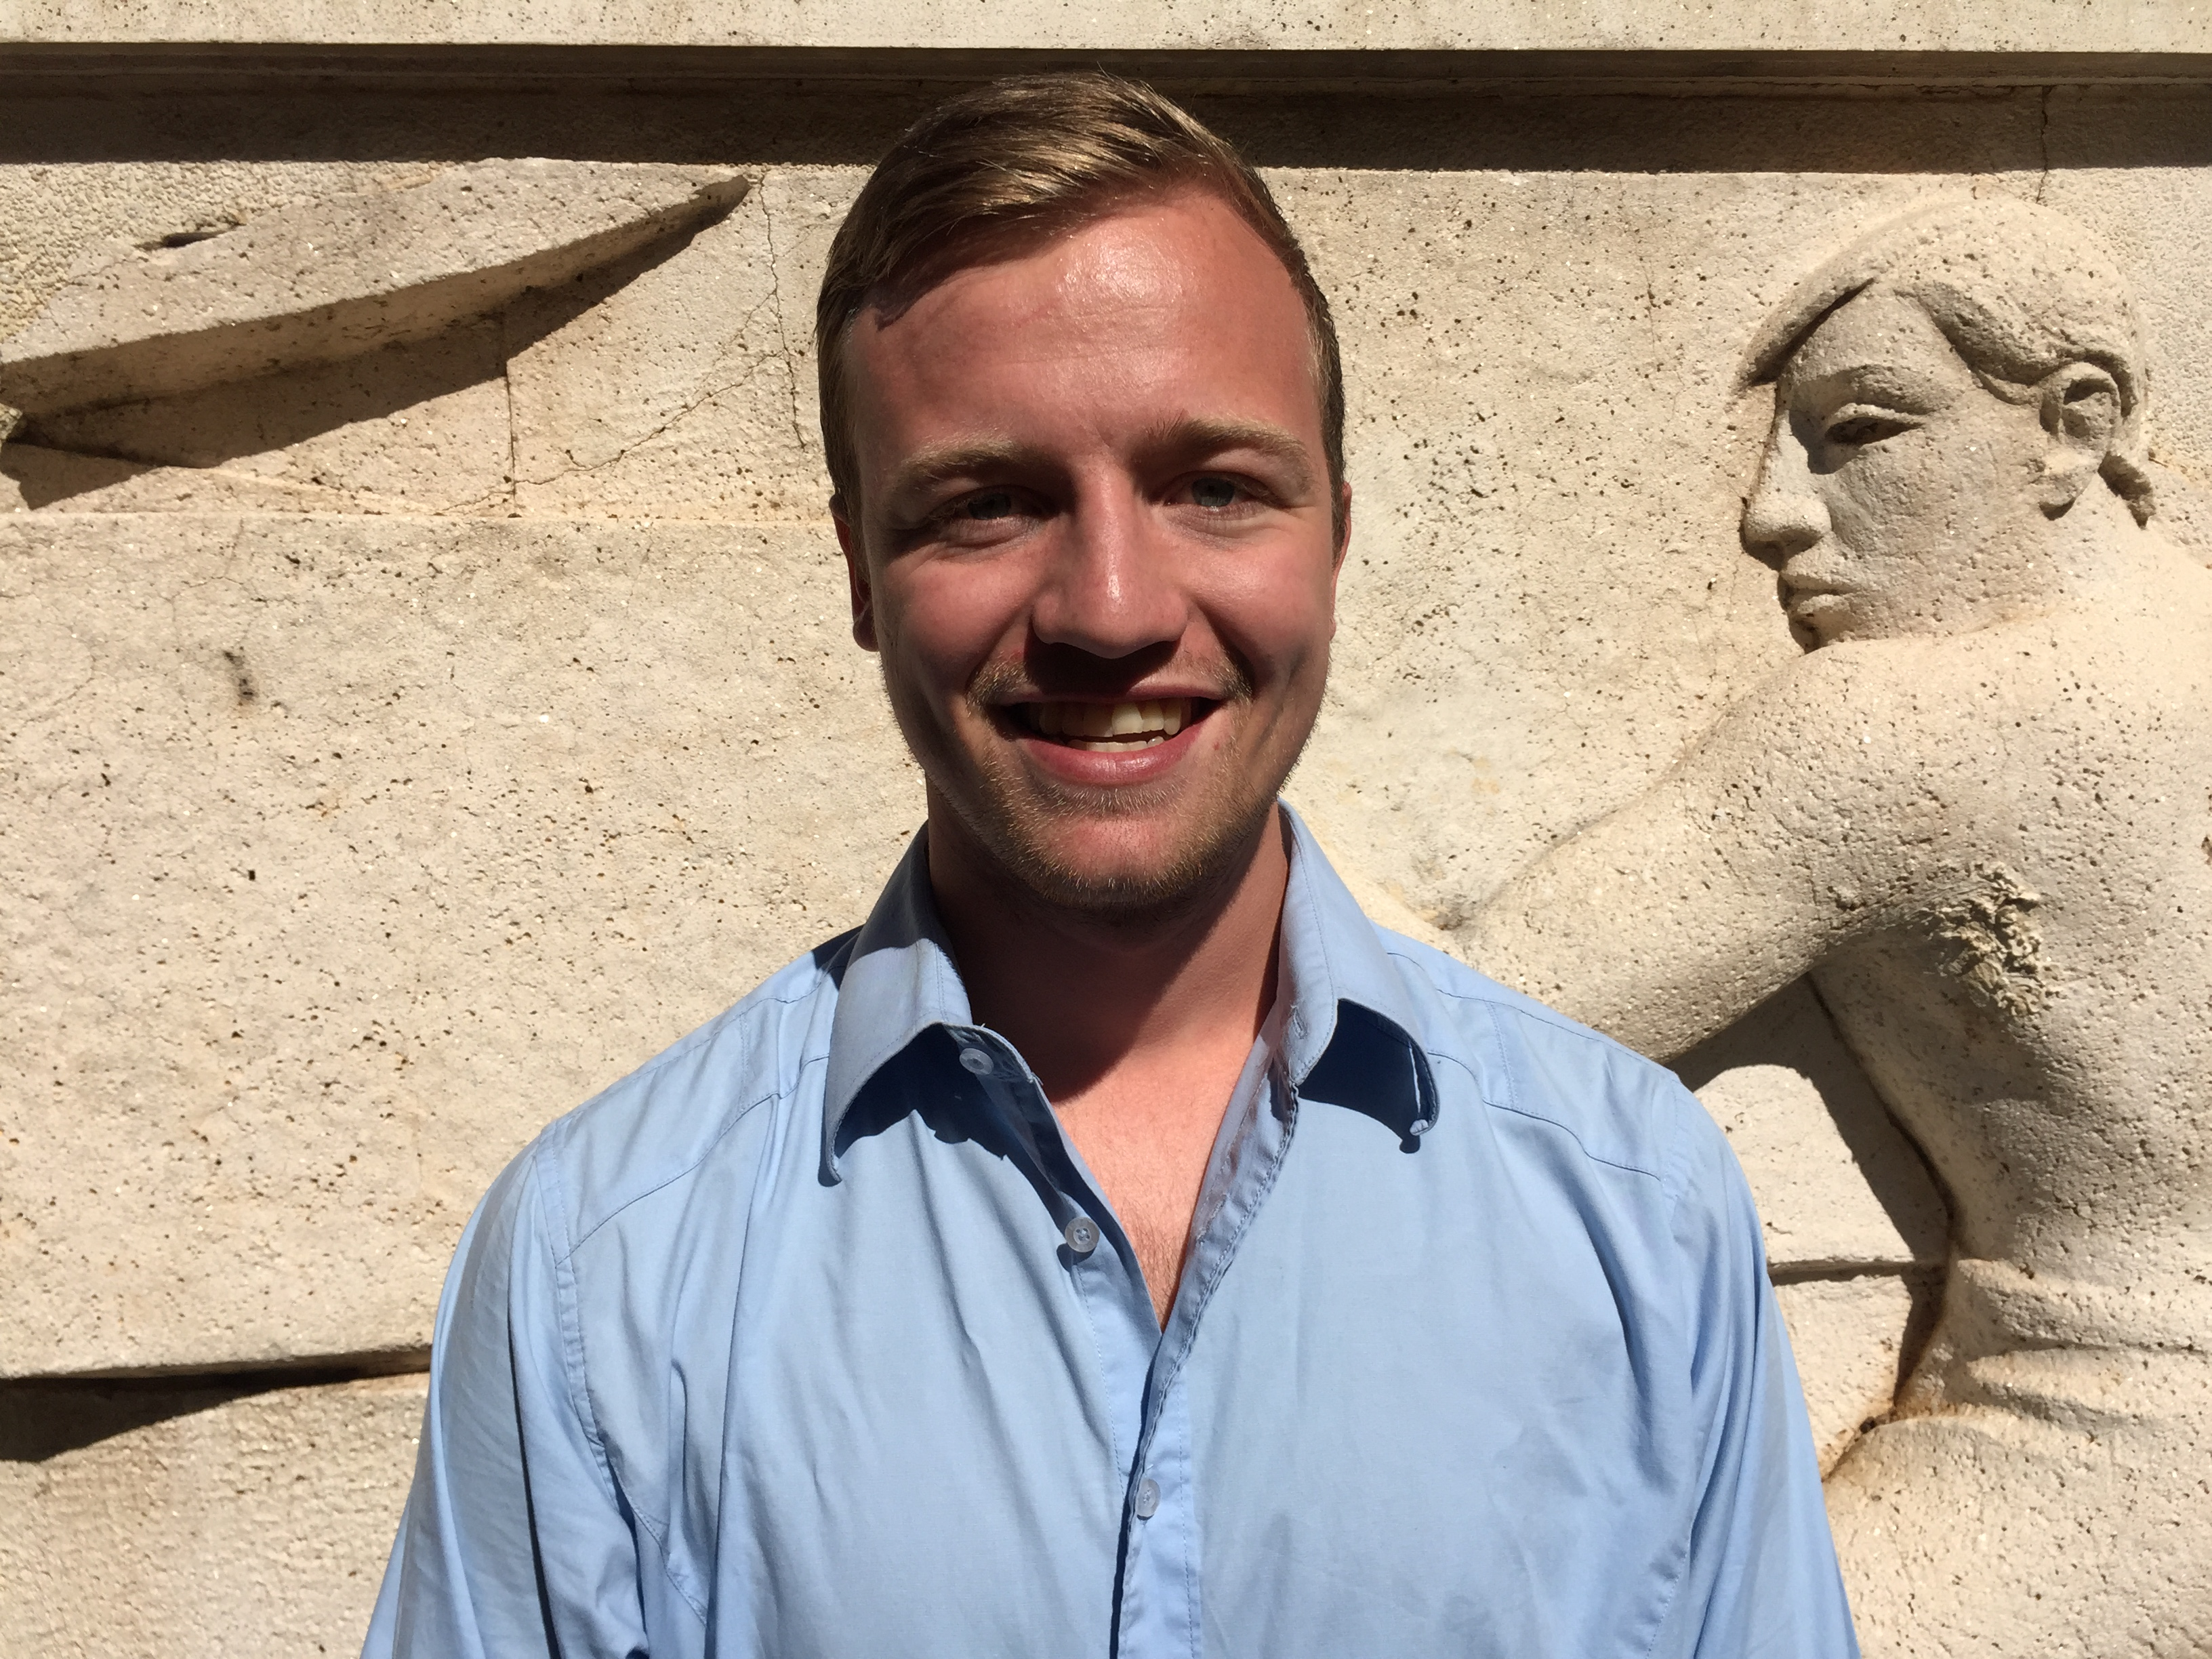
\includegraphics[width=\linewidth]{keagan}\\I am first and foremost career-driven. My primary aspirations in life are reaching for the highest branches of my career and having a healthy family lifestyle. While enjoying all aspects of life as a student, I still strive to always consider my future successes in society and the impact that any actions I commit may have on others as a result. Whilst acknowledging that it is necessary to help others to the best of my ability in advancing their own lives, I take a larger interest in ensuring a secure, comfortable lifestyle for myself. The technological environment has captivated my interest from a very young age and my fixation on developing technology that will help the human race in experiencing a more enjoyable life is a testament to that. It is through software development that I hope to leave my legacy in this world, since I see this as the most effective way for myself to leave this world in a better state than I found it. I am eager to tackle new challenges and pride myself on the fact that I am always able to find a solution to a problem. It is for this reason that I can describe my approach to programming using the expression "Where there is a will, there is a way". Although I am confident of my abilities as a software developer, I respect the fact that there are people who have a much broader knowledge of the field than I do and am willing to learn from these people in order to further my own experience.
\end{multicols}

\spacedhrule{0em}{-0.4em}

\roottitle{Experience}

\headedsection
  {\href{http://www.bbd.co.za}{Barone, Budge \& Dominick (Pty) Ltd}}
  {\textsc{Houghton Estate, Johannesburg}} {%
  \headedsubsection
    {Bursar}{Jan\apo13 -- present}
    {\bodytext{BBD implements and maintains complex business systems. A customer with a requirement for custom software, which must fit into their business, and must meet the business goals approaches BBD with the goal in mind of obtaining a software solution thereof.\\}}
    }
    
\spacedhrule{-0.2em}{-0.4em}


\roottitle{Technical Skills}

\inlineheadsection  % special section that has an inline header with a 'hanging' paragraph
  {Technical expertise:}
  {Software development aspects including software design patterns, data algorithms and programming fundamentals (Novice). I have experience in Delphi (4 years), Java (3 years), C\# (3 years), C++ (1 year) and SQL (2 years).  I also have a wealth of experience with web technologies such as \acr{HTML}, \acr{XML}, and JavaScript (Angular, NodeJS, BootStrap, jQuery). Additionally, I have a moderate knowledge of various Artificial Intelligence concepts and an extensive experience in Information System modelling.}

\vspace{0.5em}
\inlineheadsection
  {Natural languages:}
  {English \emph{(mother tongue)}, Afrikaans \emph{(full professional proficiency)}, Greek \emph{(elementary proficiency)}.}


\spacedhrule{1.6em}{-0.4em}

\roottitle{Interests}
\inlineheadsection
  {Non-exhaustive:}
  {Technology, Sports (Rugby), Socialising, Outdoors, Gaming, Travelling}

  
\spacedhrule{1.6em}{-0.4em}  
  
\roottitle{Non - Technical Strengths}

\inlineheadsection
  {Social skills:}
  {I am a person who has a witty sense of humour. I see myself as the forerunner of my group of friends and am always keen to organise a get-together at my place of residence. In terms of meeting new people, I portray my true self because I believe in always being who I am, and I have been in contact with many different kinds of people so I have a good understanding of communication with most people.}
\inlineheadsection
  {Professional skills:}
  {I always try my best to be punctual and to have work completed by the deadline as this is the only way a group will be able to complete a project effectively and I like to consider actions carefully in conflict situations rather than force my own ideas upon others.}
  
\spacedhrule{1.6em}{-0.4em}  
  
\roottitle{Why CSIR Ironman Image Throw Thingy?}

\inlineheadsection
  {Because:}
  {App development is one part of IT I have yet to get into properly and since it is becoming a big part of the technological world today, I hope to use this project as an opportunity to expand my knowledge in this respect. I also wanted to do a project that would push my boundaries a lot and this Iron Man project seems like the most futuristic one.}